%!TEX root = paper.tex
%%%%%%%%%%%%%%%%%%%%%%%%%%%%%%%%%%%%%%%%%%%%%%%%%%%%%%%%%%%%%%%%%%%%%%%%%%%%%%%%
\section{Background}
\label{sec:background}

We now introduce some fundamental terms and concepts such as tickrate, framerate, command message rate, and end-to-end lag in Section~\ref{subsec:game-model} through \ref{subsec:e2e-lag}. Then, Section~\ref{sec:measurementapproaches} presents various lag measurement techniques.


%%%%%%%%%%%%%%%%%%%%%%%%%%%%%%%%%%%%%%%%%%%%%%%%%%%%%%%%%%%%%%%%%%%%%%%%%%%%%%%%
\subsection{Basic Game Model}
\label{subsec:game-model}


At their core video games are essentially feedback-directed real-time simulators. Figure~\ref{fig:gameloop1} overviews a simplified simulation loop consisting of three parts.
The game reads player input, updates the game state, and renders new screen contents. This loop repeats as long as the game is running. While the three parts are interrelated, and every component provides some form of input to the next, they may still proceed at their own intrinsic paces. (For example, the state of the game world is updated even if the player character does not move.)In this simplified model, we distinguish a generic process for player input, a \textit{tickrate} that governs the frequency of game state updates, and a \textit{framerate} determining how often the screen is updated every second.

Note that actual game implementations sometimes choose to update parts of the game state on different fixed frequencies. For example, a physics effect that does not influence gameplay directly could be updated at only half the tickrate. Also, the parameters of the player input process depend on the game genre and on the player action currently performed. Please refer to Table~\ref{tbl:tickrates} for exemplary rates of current games.

%Popular examples for the fixed tickrates of game servers include \SI{64}{\hertz} or \SI{128}{\hertz} for \textsc{Counter-Strike: Global Offensive}, \SI{20}{\hertz} for \textsc{Minecraft}, or \SI{30}{\hertz} for \textsc{Dota 2}.



%%%%%%%%%%%%%%%%%%%%%%%%%%%%%%%%%%%%%%%%%%%%%%%%%%%%%%%%%%%%%%%%%%%%%%%%%%%%%%%%
\subsection{Game Architecture Flavors}
% TODO: needs a better word than types, more like architectures. Feedback welcome
% TODO: need to find a better word than game (delivery) flavors

We next discuss how different implementations of game architectures set the local/remote boundary, as depicted in Fig.~\ref{fig:component-models}. Consider first a \textit{single-player game} (sub-figure \textit{a}), with all of the components running locally. However, we previously mentioned that the three parts of the main game loop each progress at individual paces. Therefore, one may conceptually separate server-side input and state management components out of the single-player architecture, and thus form an \textit{online video game} (sub-figure \textit{b}). Now, player state information is transmitted to the game server across the network, and likewise, state updates from the server transit the network until they reach the game client.
Furthermore, the game server can be the central, authoritative point of state synchronization for other connected clients.
It should be noted that for reasons of network and processing efficiency, player input events are usually batched, and sent to the server according to a specific \textit{command message rate}.

%\textit{Online video games} (i.e. mostly multiplayer games) complicate this update logic a bit as seen in the depiction of Fig~\ref{fig:component-model-online}. In client/server online games, the client is not the final authority over its game state any more. Instead, interpreted input commands are sent to the server and a preliminary game state is calculated locally. When the authoritative update from the server is received the two states can be once again be synchronized.

In a different possible separation of components, the game client (which includes state management and rendering) is situated on a remote entity. This gives rise to \textit{cloud gaming} (sub-figure \textit{c}), which is a form of \textit{game streaming} where the game streaming server is part of a larger streaming service hosted at a data center. Due to the spatial separation of the input/output devices and the game engine, input data needs to be sent from the streaming client to the game engine. The return channel does not transport game state messages in this scenario, but rather streams the rendered audio and video data.

%Fig.~\ref{fig:tickrate-streamed} gives again an overview of all these components for a combined streamed online video game scenario by highlighting the involved entities and interaction triggers in more detail.

% \begin{figure*}[!t]
%   \centering
%   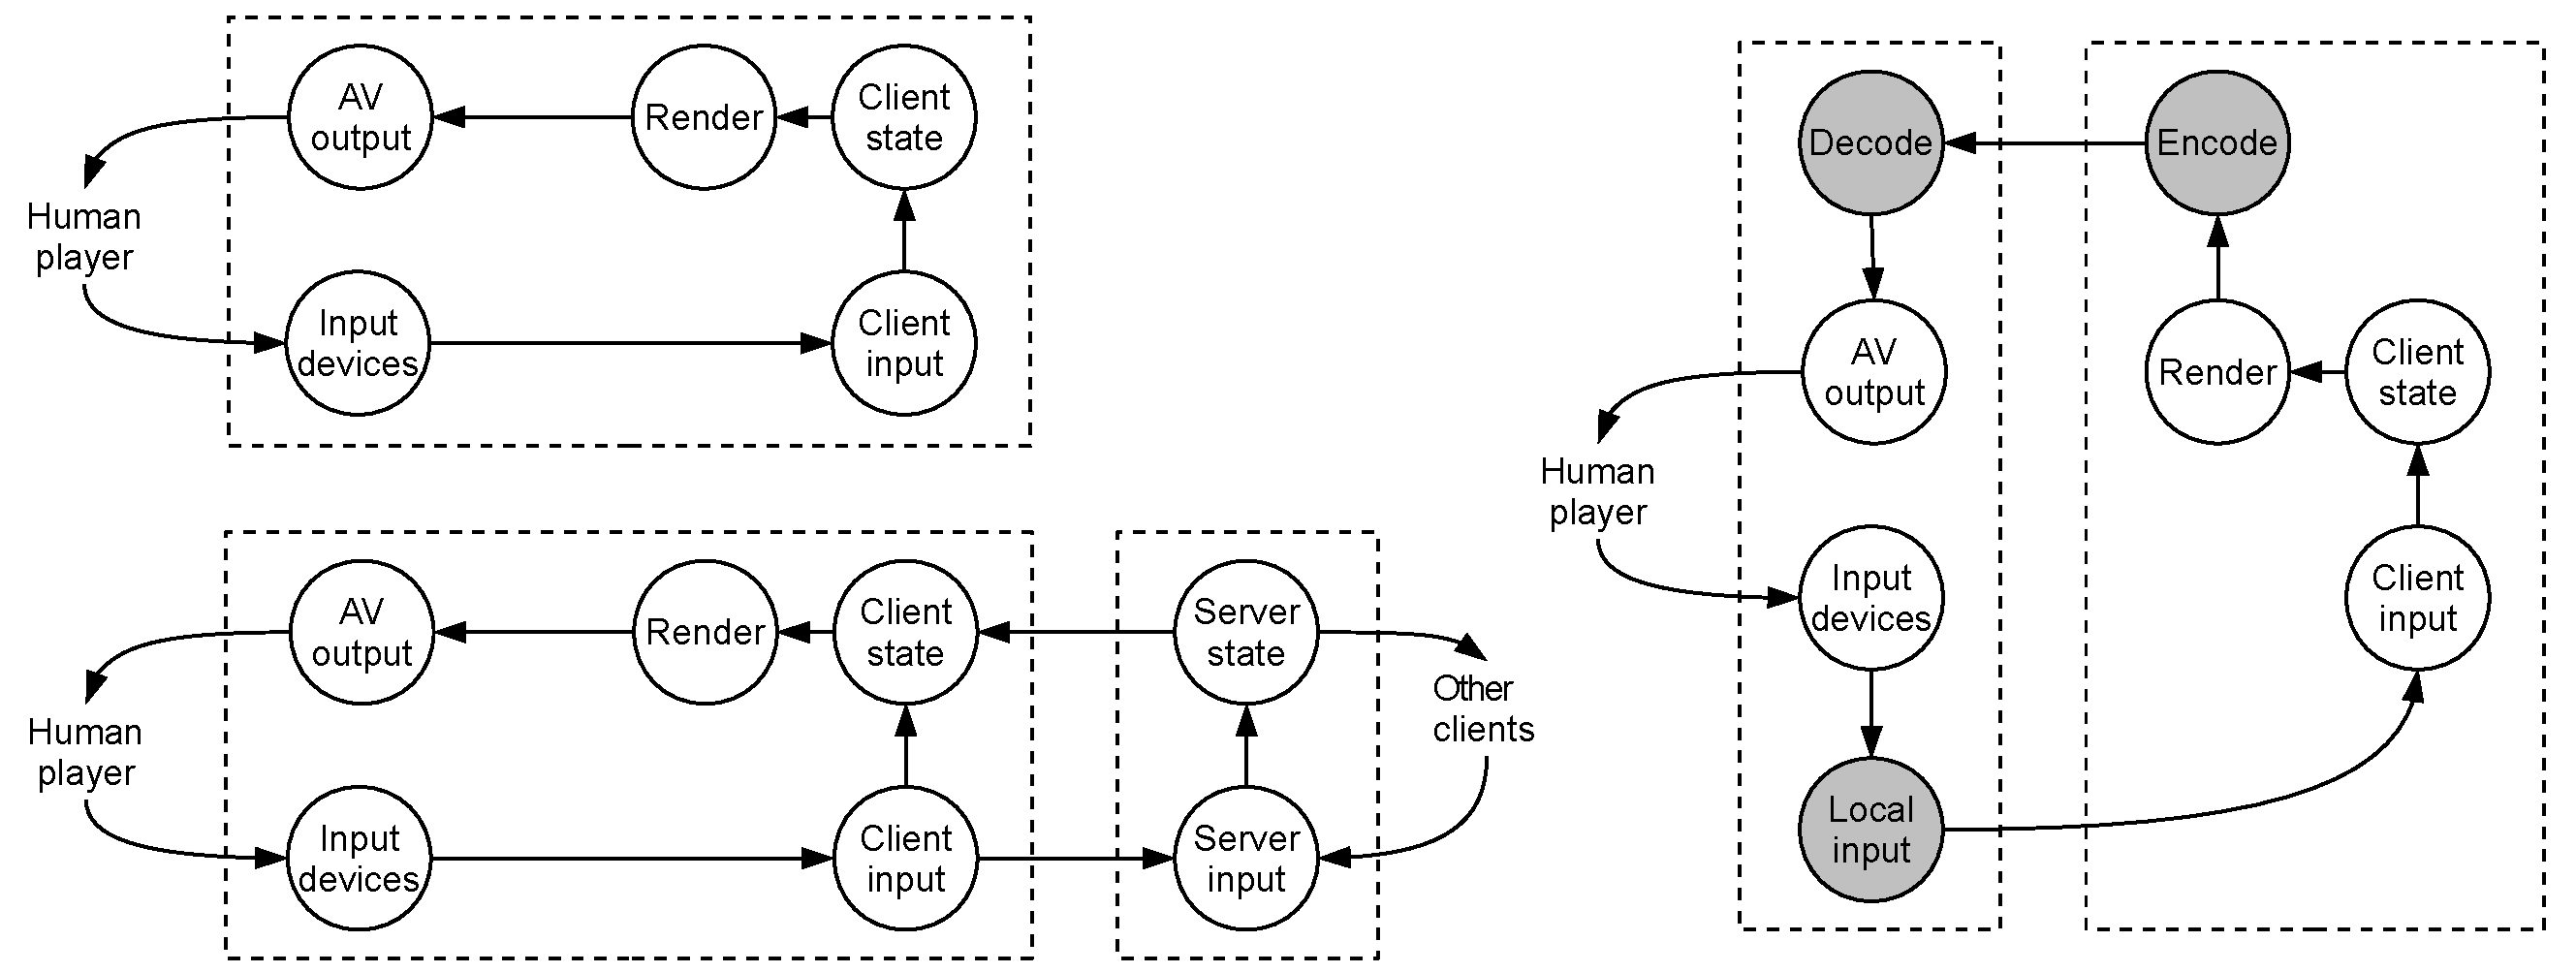
\includegraphics[width=0.9\textwidth]{../../models/component_interaction_full.pdf}
%   \caption{Interactions between components in different video game models. \textit{(a)} Single-player, \textit{(b)} online, \textit{(c)} cloud game.}
%   \label{fig:component-models}
% \end{figure*}

%%%%%%%%%%%%%%%%%%%%%%%%%%%%%%%%%%%%%%%%%%%%%%%%%%%%%%%%%%%%%%%%%%%%%%%%%%%%%%%%
\subsection{Framerate}
\label{sec:framerate}

In contrast to traditional video media that play back at fixed framerates, e.g., \SI{24}{\hertz}, video games are more flexible but also much more demanding on the framerate. First, the framerate in a game may fluctuate as the processing time of the render process depends on the scene complexity.
Then, video games usually target higher framerates than other media do: \SI{30}{\hertz}, \SI{60}{\hertz}, or even \SI{120}{\hertz}, depending on the type of game. Higher framerates enable smoother camera movement and scene transitions, as games often present faster scenes when compared to videos; they also help in increasing the interactivity as video games constantly require input on short time scales to which the game reacts and displays the feedback. Therefore, the framerate influences the reactivity of a game, but can also be a source of latency itself.


%%%%%%%%%%%%%%%%%%%%%%%%%%%%%%%%%%%%%%%%%%%%%%%%%%%%%%%%%%%%%%%%%%%%%%%%%%%%%%%%
\subsection{End-to-End Lag}\label{subsec:e2e-lag}

Lag in video gaming is often described solely on the basis of the network delay in an online game. It should be evident that the lag is a critically important factor for almost all games. This is especially true for fast or competitive games, as it governs the reaction time to in-game events.

However, focussing solely on network delay neglects other components that contribute to the lag, including the input device, the time to sample and process the input, the game engine and server and their tickrates, frame rendering time, and ultimately the time to display the frame on the monitor. Only if all sources are factored in the complete \textit{end-to-end lag} is captured. Notably, this lag is usually not constant but can vary depending on the type of action triggered by the input. While some simple actions, say opening the menu, may have a very short lag, more complex interactions, e.g., issuing command that moves the player character in the game world, may take considerable longer to complete. %, partly due to the actions taking more than one game tick to complete.
Therefore, each video game will have a distinct ``lag profile''.


% TODO:
% This subsection adds the player to the architectures introduced above, highlights potential QoS and QoE (or discusses why some chosing a particular QoE metric is not useful) metrics to study. At the end of this section, the reader should agree that end to end latency is a sensible starting point to study video game qos.


%%%%%%%%%%%%%%%%%%%%%%%%%%%%%%%%%%%%%%%%%%%%%%%%%%%%%%%%%%%%%%%%%%%%%%%%%%%%%%%%
\subsection{Measurement Approaches}
\label{sec:measurementapproaches}

%With the central role of the end-to-end lag in mind, it is natural to assume that this
Lag also plays a critical role in both subjective and objective video game quality assessments. Therefore, the end-to-end lag needs to be correctly examined and quantified from any kind of video game. Unfortunately, video games usually represent a black box with very few possible vantage points where measurements can be taken. Below we discuss three distinct methods which are each situated at unique vantage points as depicted in Fig.~\ref{fig:measurement-methods}.
The methods described below are ordered roughly from lowest to highest complexity of implementation.

\begin{figure}[!t]
    \centering
    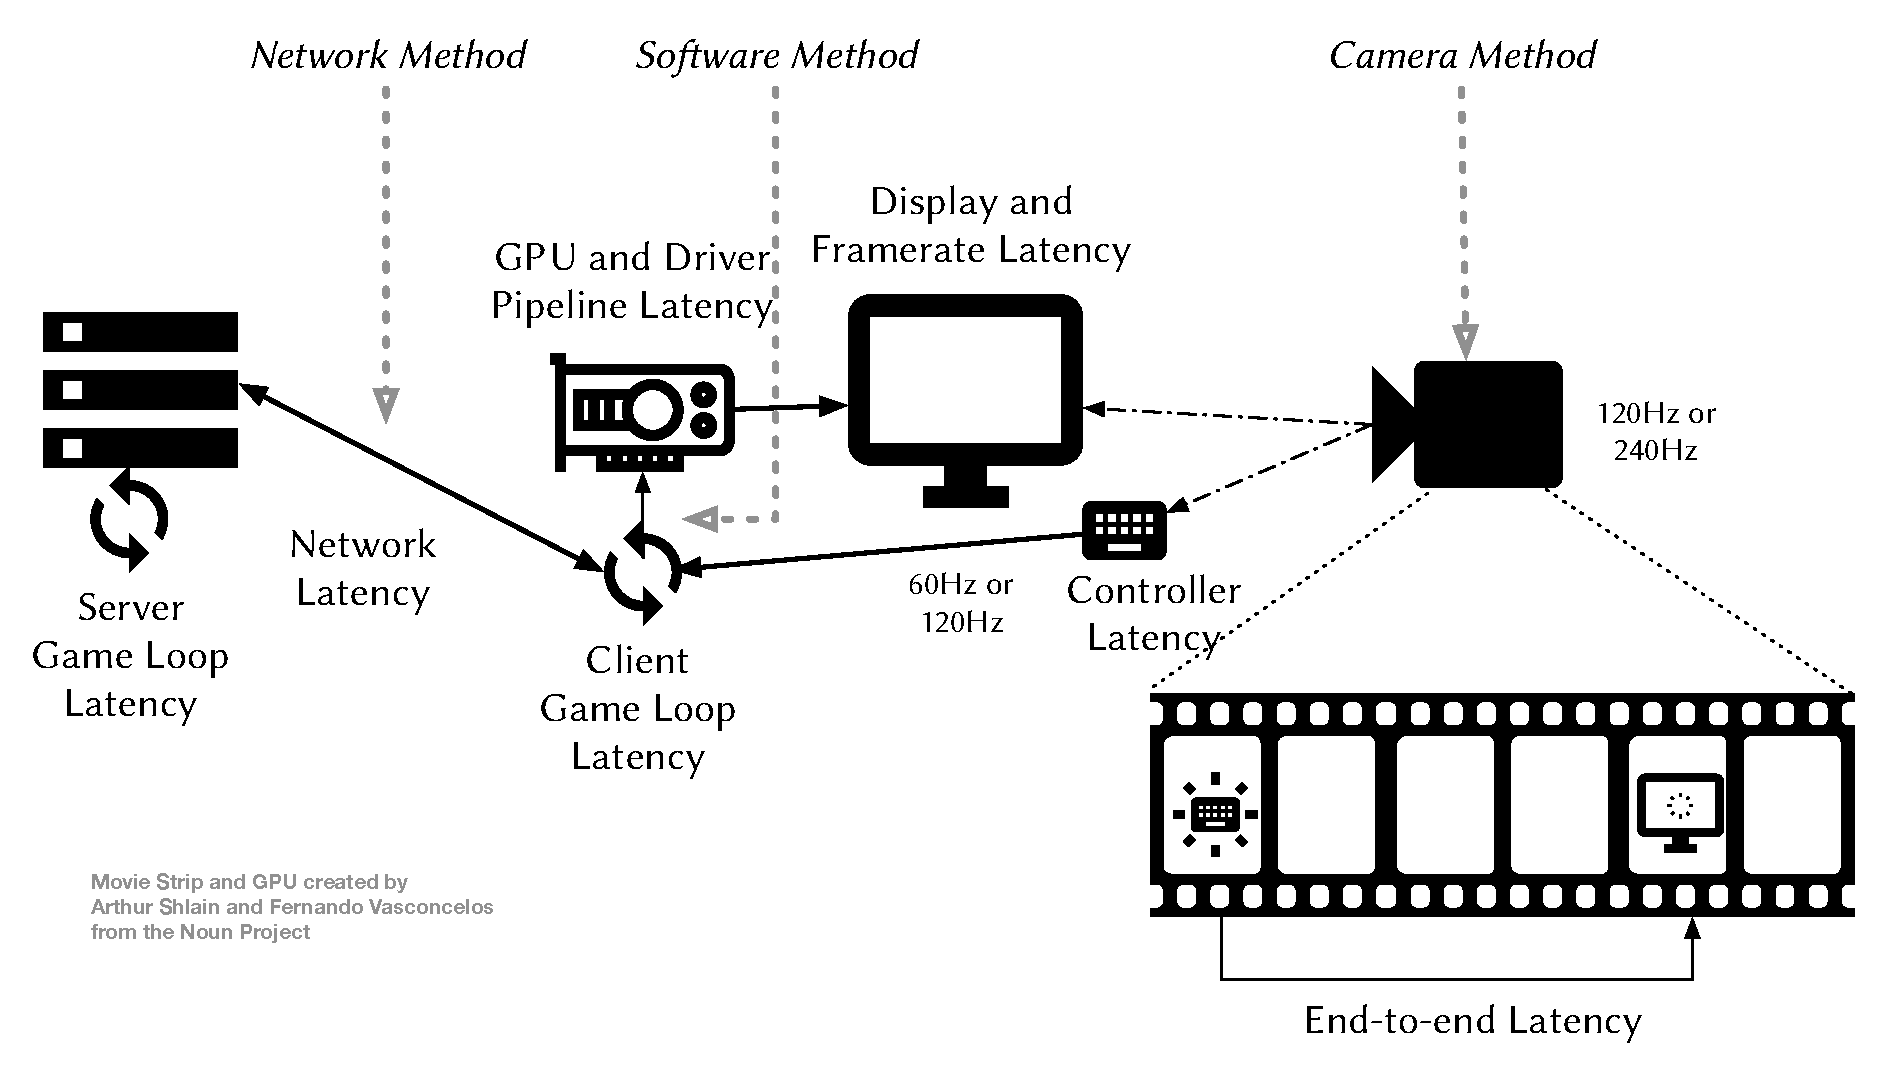
\includegraphics[width=1.0\columnwidth]{../../models/e2e-lag.pdf}
    \caption{Location of three measurement approaches to capture end-to-end lag in an online video game.}
\label{fig:measurement-methods}
\end{figure}


%%%%%%%%%%%%%%%%%%%%%%%%%%%%%%%%%%%%%%%%%%%%%%%%%%%%%%%%%%%%%%%%%%%%%%%%%%%%%%%%
\subsubsection{Screen Recording Software Method}
Recording in software the output stream of a video game might be the simplest approach to determine video game lag. It can capture both the framerate and \gls{IAT} at a driver level, and the recorded video can be used for image and quality analyses as well as to correlate it to additionally recorded input events in order to calculate the lag. This is not the complete end-to-end lag however, as both the controller and screen output delay are missing. The need to install additional software might make it unsuitable for some scenarios, e.g., when measuring console video games. As a variant of this method, one can also record the output stream with a video capture card on a secondary computer, which does not negatively effect the game's performance as the software method would.

Examples of this approach include both \cite{Chen:2011:MLC:2072298.2071991} and \cite{6670099} which measured the latency of cloud gaming services in the game client. They do this by invoking the system menu in games and measuring the time until it is displayed. A 2013 paper \cite{6574660} investigates the quality of cloud gaming interactiveness (i.e., the lag) as well as image quality by employing software recording methods on the client's computer.
%However, this method assumes a constant delay of game actions and may not capture the actual end-to-end lag of many of real game actions, as they are typically different from and longer as the latency of displaying a menu. A 2013 paper \cite{6574660} investigates the quality of cloud gaming interactiveness (latency) as well as image quality by employing software recording methods on the client's computer. With these techniques the challenges regarding the quality are discussed.


%%%%%%%%%%%%%%%%%%%%%%%%%%%%%%%%%%%%%%%%%%%%%%%%%%%%%%%%%%%%%%%%%%%%%%%%%%%%%%%%
\subsubsection{Passive Network Measurements}
In some cases it may also be advantageous to tap into the network interactions of the games and record the command and update messages sent between server and clients. While this is not a direct measure of game quality, it can give insights into the game's inner workings, such as the tick rates, and one can derive, e.g., the lowest achievable end-to-end lag from this.

%Can only investigate command and update messages, not tick rate directly. Evaluate rate, IAT, and bandwidth, estimate latency (though there may be no direct link between commands and updates).

% Besides simple flow-based or packet-counting network metrics, many games also allow for deeper packet-dissecting analyses, as the often rely on standardized protocols or data formats, such as Protobuf\footnote{\url{https://developers.google.com/protocol-buffers/}} or incorporate well-known third-party multiplayer-enabling libraries. %And cloud games sometimes use derivates from the RTP-family or XMPP-based(VERIFY) protocols. 
% Additionally, almost no game encrypts its time-critical messages, enabling an easy read-out. Through these means, the specific commands can be read from the network and potentially linked to their effect on the game state in the corresponding state update messages.
%, but also potentially allowing malicious actions to be taken easily.


%%%%%%%%%%%%%%%%%%%%%%%%%%%%%%%%%%%%%%%%%%%%%%%%%%%%%%%%%%%%%%%%%%%%%%%%%%%%%%%%
\subsubsection{Camera Recordings}
Finally, the only method to fully capture the end-to-end lag is to simultaneously record both the screen and input device through an external measurement device like a video camera.
%\hoss{Mit 'only' ware ich vorsichtig. Es kann auch noch andere Moeglichkeiten mittels physikalischer Sensoren geben, evtl. sowas \cite{di2010new} also aehnlich zu \cite{beyermethod}. Evtl sollte man 'Camera Recordings and Sensoring' schreiben?}
The experimenter then counts the frames between pressing a button on the input device and the action appearing on the screen and calculates the lag from this. For better visibility the input device is usually modified with an LED that turns on when the button is pressed.
%Also, the camera should operate at least at twice the monitor's refresh rate according to the Nyquist-Shannon sampling theorem.
An additional benefit of this method is that the game and the computers remain unaltered and are therefore not affecting any properties of the game. A variant of this approach, replacing the camera with a photodiode and synthetically creating the input events with a microcontroller is described in \cite{beyermethod}, though it may be difficult to use for certain game actions that have a barely visible or unpredictable on-screen effect.




%%%%%%%%%%%%%%%%%%%%%%%%%%%%%%%%%%%%%%%%%%%%%%%%%%%%%%%%%%%%%%%%%%%%%%%%%%%%%%%%
\subsection{Related Work}

The assessment of video games has been a topic in many past papers. Due to the strong interactivity of games and the large number of different game mechanics most of the research is focused on conducting user studies and noting the subjective quality of the users. The outcome of these studies depends strongly on a wide selection of factors (e.g., on the precise setup, the game, and the choice of players) which makes comparing their results quite difficult. This section presents a few examples of such studies.

In \cite{5976180} Jarschel et al. identify some influence factors on the subjective quality of cloud gaming through a user survey for certain games and three different game categories (slow, medium, fast games) that have been subjected to worsening \gls{QoS} parameters. Downstream packet loss and delay was noted be be especially problematic for achieving a good quality. Similarly, the authors of \cite{4591393} observed the relationship of players quitting a \gls{MMO} game with deteriorating \gls{QoS} and noted an impact proportion of 1:2:4:3 for delay, jitter, and packet loss on both the client-to-server and server-to-client connections respectively. Additionally, a user study in \cite{4604397} also showed a correlation of the \gls{QoE} to the delay as well as the jitter for another \gls{MMO}, in this case the total delay had more impact than the delay variation. Regarding the subjective quality in first person shooters, the authors of \cite{6614351} find a strong impact of the delay and packet loss on the experienced quality. The authors of \cite{6404025} and \cite{beyerusing} use \gls{fEMG} and \gls{EEG} approaches respectively to examine individual gamers' reaction to various cloud games and measure the quality they are experiencing in terms of real-time strictness and \gls{QoE}. Finally, an ITU-T Recommendation \cite{mollertowards} concerning subjectively measuring video game \gls{QoE} is also in preparation, which discusses game-relevant \gls{QoS}-metrics as well as the selection of players and games.

In order to avoid some of the issues with subjective user studies, other approaches examine the player objective performance through in-game metrics such as the game's highscore or the duration to achieve a certain task. For example, a user study in \cite{Chen:2006:SOG:1167838.1167859} observes a decrease in the objective quality assessment metrics (the playing duration) in an \gls{MMO} due to the influence of network factors. A 2006 paper \cite{Claypool:2006:LPA:1167838.1167860} categorizes player actions and their relationship to latency, with special regards for the precision and deadlines of actions. However, the in-game metrics under study can not represent short-term effects of latency as they operate on much larger time-scales. 
%(e.g. researching the whole technology tree in Warcraft 3 is neither a representative action of the game nor delay-sensitive at all). Also the presence of lag compensation techniques is not considered. The end result is a delay tolerance table which probably is not very representative of modern video games.
A second paper by Claypool et al. \cite{claypool2007} furthers this notion of the influence of network \gls{QoS} on in-game actions and specifically looks at player performance in first person games. A user study records the performance in artificially created in-game environments. Here, the performance gets worse with a degraded network, albeit at a very slow pace. %Players were also subjected to very low framerates of \SI{7}{\hertz} and \SI{3}{\hertz}, which is such an unrealistic setting, that it should not even have been tested. The reasons for this are laid out in Section~\ref{sec:framerate}.
The ``kills per minute'' of normal players in the \gls{FPS} \textsc{Quake 3} are investigated by \cite{1266180}, which sees a steady decline of this subjective performance metric when increasing the network delay. However, another paper \cite{Beigbeder:2004:ELL:1016540.1016556}, looking at player performance in \textsc{Unreal Tournament 2003} in a controlled in-game environment, finds almost no influence of increased delay and packet loss, even at high values of \SI{200}{\milli\second}. %The discrepancy between the otherwise similar studies could potentially be attributed to the specific construction of the in-game test environment. 
A 2002 paper \cite{Pantel:2002:IDR:507670.507674}, which gathered objective \gls{QoE} measurements from a custom-made RC racing video game, again sees a strong dependence of the player's performance on the delay, and suggests that a network \acrshort{RTT} of \SI{200}{\milli\second} is barely usable and \SI{500}{\milli\second} completely unusable. Finally, the authors of \cite{Bredel:2010:MSR:1944796.1944797} also find a strong and negative influence of high delay on the player's performance, in this case again in \textsc{Quake 3}. 

It is interesting to note the discrepancies between the studies both in terms of the influencing parameters as well as their degree. Considering the complexity and variability of video games and the difficulties of finding and setting up good comparable scenarios and testbeds, it is understandable that some studies come to different results. This makes it much more important to understand the basic components and underlying objective metrics better. Quality estimations of video games could be much more representative if models for these metrics would exist to easily understand their influences without having to conduct a full user study.





%Pure \gls{QoS} views on the quality of online video games are rather are, but are nonetheless important in correctly assessing any game-related parameters and are also the foundation for most objective and subjective \gls{QoE} studies.



%A 2012 article notes the dependence of gaming on latency and the difficulties cloud-based solutions have in providing a sufficiently low latency. The suggest a move closer to the edge to reach more users in a quality they deem adequate.  \cite{Choy:2012:BSC:2501560.2501563}.
%``The Brewing Storm in Cloud Gaming: A Measurement Study on Cloud to End-user Latency'' 

%``Placing Virtual Machines to Optimize Cloud Gaming Experience'' \cite{6853364}  interesting for cloud gaming economics

%Adaptive Mobile Cloud Computing to Enable Rich Mobile Multimedia Applications \cite{6413270}

%Addressing Response Time and Video Quality in Remote Server Based Internet Mobile Gaming \cite{5506572} optimize mobile cloud gaming based on a certain impairment function and by reducing video bitrate and fps (even sub 10fps...)

%``Kahawai: High-Quality Mobile Gaming Using GPU Offload'' \cite{Cuervo:2015:KHM:2742647.2742657}

%``Outatime: Using Speculation to Enable Low-Latency Continuous Interaction for Mobile Cloud Gaming'' \cite{Lee:2015:OUS:2742647.2742656}

%``Assessing the Impact of Game Type, Display Size and Network Delay on Mobile Gaming QoE'' \cite{beyer2014typedisplaydelayimpact} Another user study regarding context factors like screen size and their impact on MOS, but also game type and delay on MOS

%A Method For Feedback Delay Measurement Using a Low-cost Arduino Microcontroller \cite{beyermethod} already covered in measurement methods section

%``QoE Assessment of Interactivity and Fairness in First Person Shooting with Group Synchronization Control'' \cite{Ida:2010:QAI:1944796.1944806} interessant für lag compensation betrachtungen

%``The Impact of Video Encoding Parameters and Game Type on QoE for Cloud Gaming: a Case Study using the Steam Platform'' \cite{slivarimpact}

%``How Do New Visual Immersive Systems Influence Gaming QoE?'' \cite{hupontnew} Vergleich Immersion am monitor vs oculus. beispiel eines schlechten testsetups, da unterschiedliche FoV für beide ausgabetypen (75° vs 100°), test wird stark verfälscht

%%``An experimental estimation of latency sensitivity in multiplayer Quake 3''  vs. \cite{1266180} ``The Effects of Loss and Latency on User Performance in Unreal Tournament 2003'' \cite{Beigbeder:2004:ELL:1016540.1016556}. both papers completely contradict each other: Quake 3: significant impact of latency on game performance (kills/minute); UT3: no impact on user performance at all (kills/deaths per game)

%``Security issues in online games'' \cite{doi:10.1108/02640470210424455}








% \begin{figure}
%   \centering
%   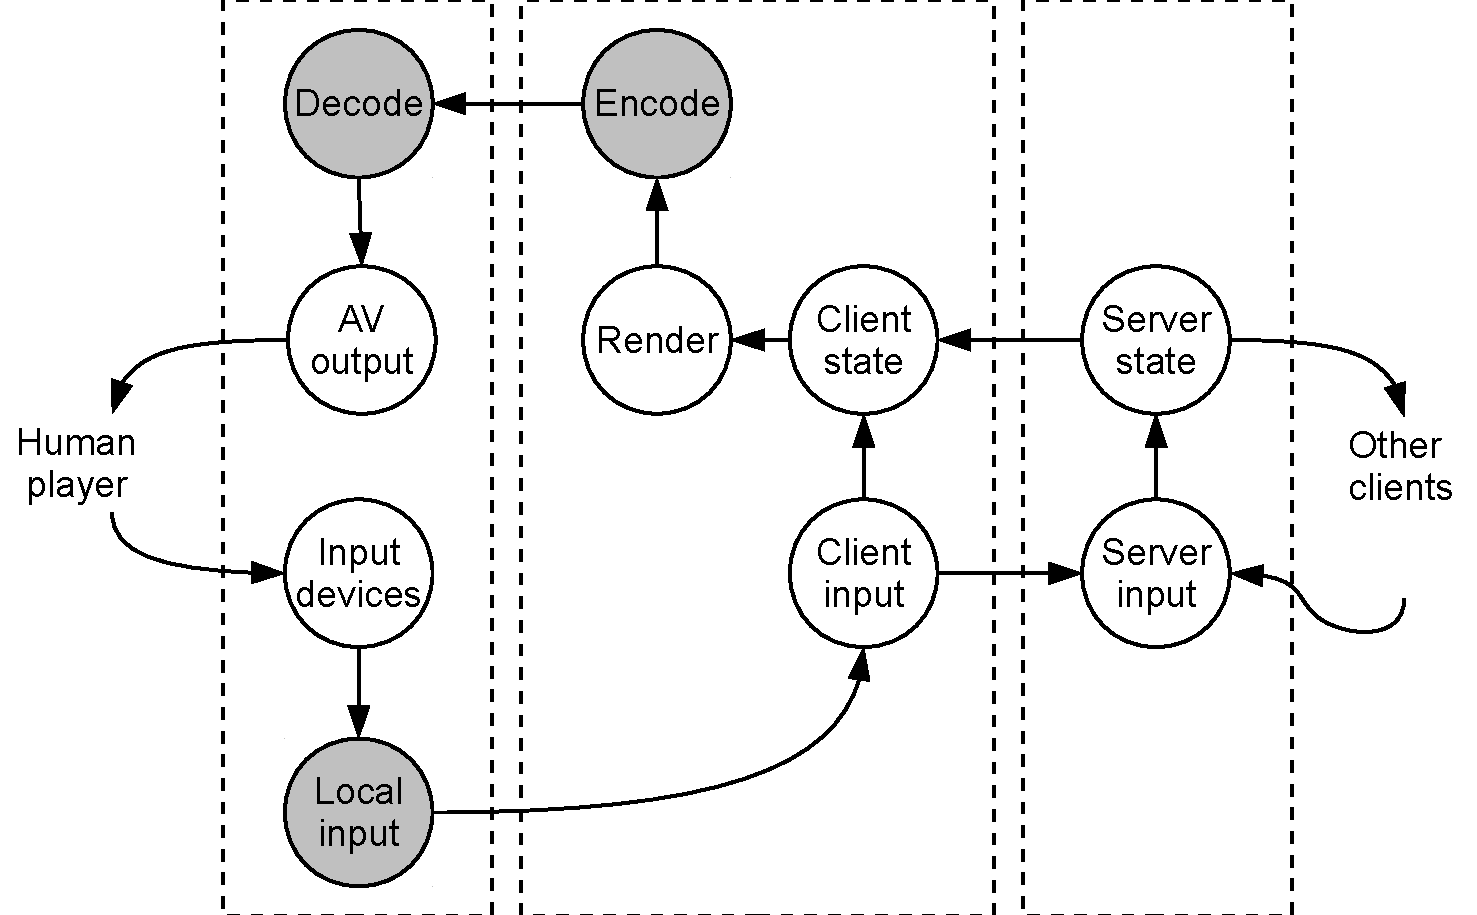
\includegraphics[width=0.8\columnwidth]{../models/component_interaction-online+cloud.pdf}
%   \caption{Interaction of TODO.}
%   \label{fig:component-model-online+cloud}
% \end{figure}

% \begin{figure}
%   \centering
%   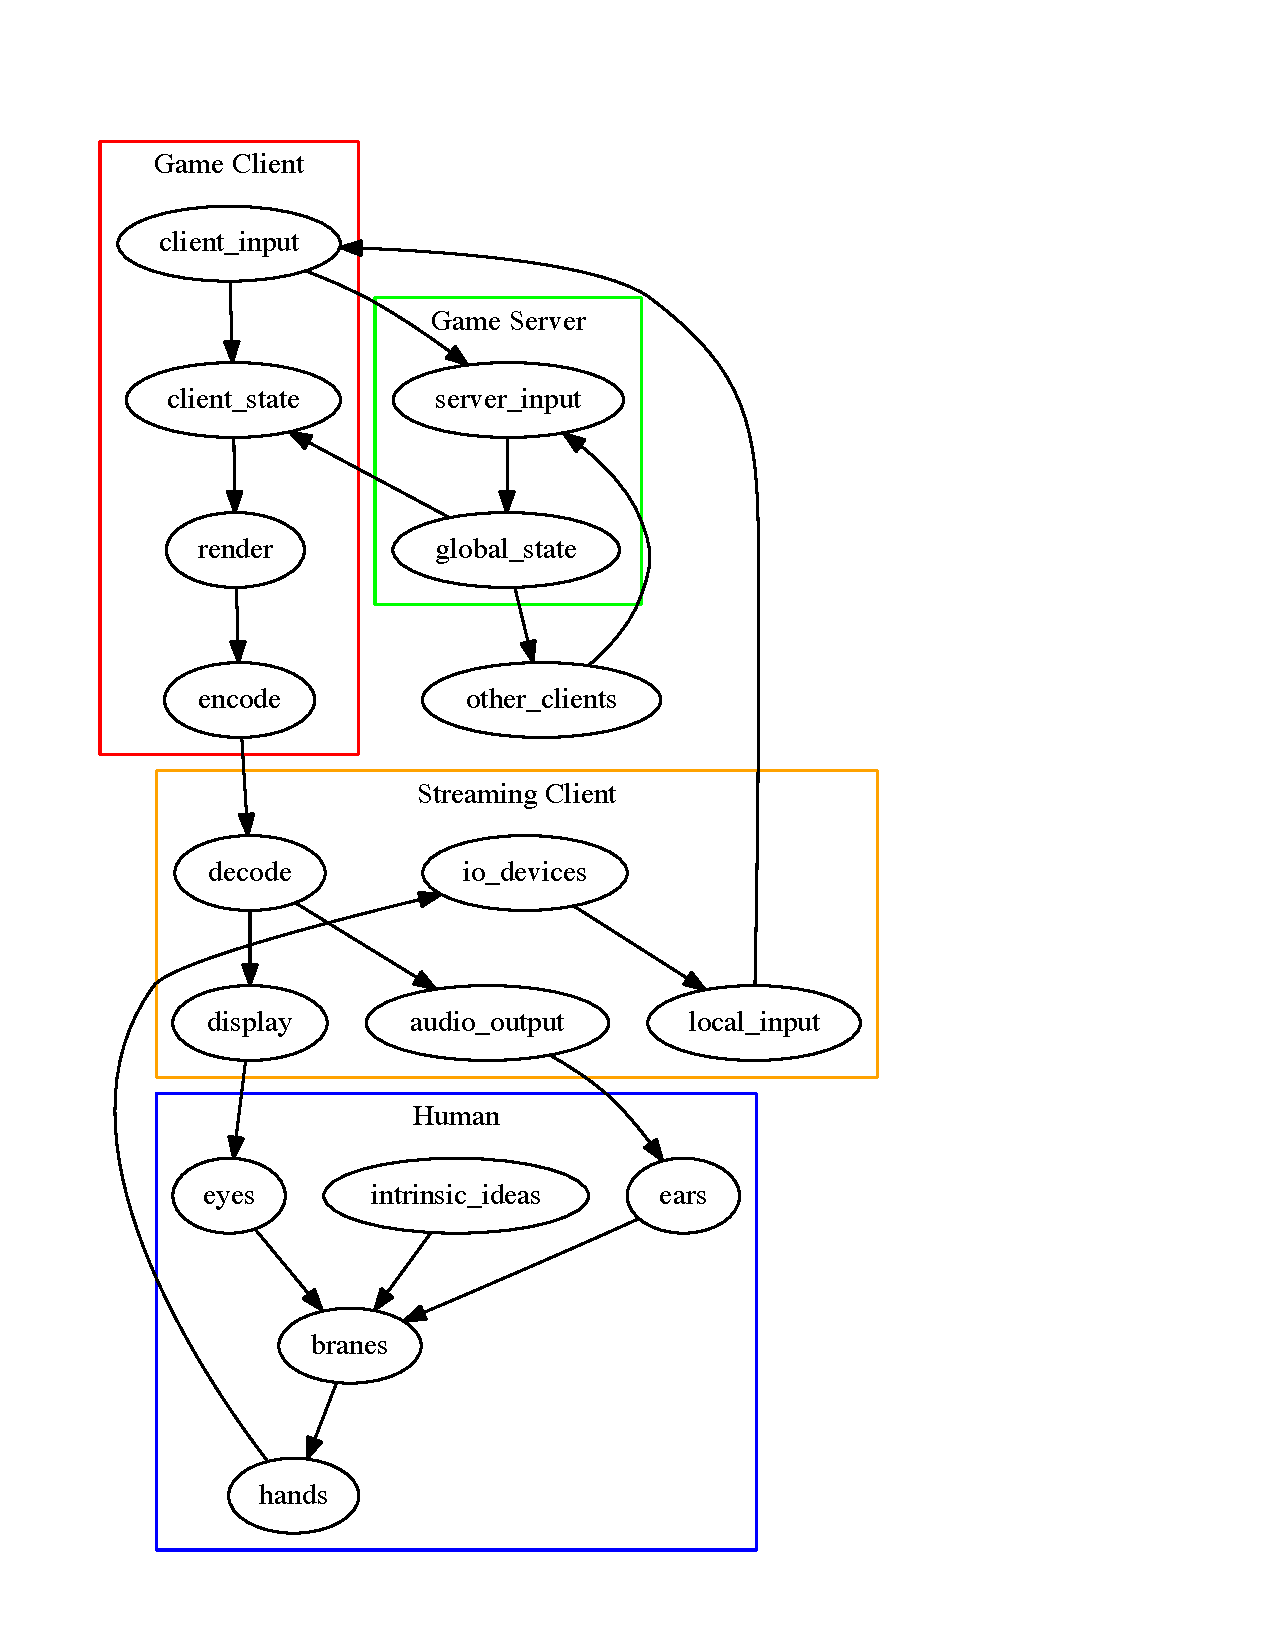
\includegraphics[width=1.0\columnwidth]{../models/cycle.pdf}
%   \caption{Interaction of TODO.}
%   \label{fig:component-model}
% \end{figure}





%Generally speaking, motion in video data is based on the principle of \textit{apparent motion}. In order to perceive objects to be in motion in videos, consecutive images have to appear at a certain rate which is considered to be at about \SI{16.67}{\hertz} according to \cite{wertheimer1912experimentelle}. Below that threshold objects will appear as two distinct objects between two consecutive frames. %This form of apparent movement is called the phi phenomenon. The higher the rate of displaying images, the more fluid the motion looks, as the discrete ``jumps'' in the position of the object get smaller the higher the framerate is.\footnote{One can verify this behavior for example at \url{https://frames-per-second.appspot.com/}.}.

% In general, there is no commonly established upper limit to the framerate that humans can still perceive as an improvement to motion presentation, the gain has however diminishing returns. The typical movie framerate of \SI{24}{\hertz} is considered to be at the lower end of motion perception but mostly still works without any problem due to the presence of motion blur. This artifact is always present in recorded images as objects are still in motion during film exposure. %A faster shutter speed reduces the amount of motion blur. % film grain also has an influence

% \begin{figure}[!t]
% 	\centering
% 	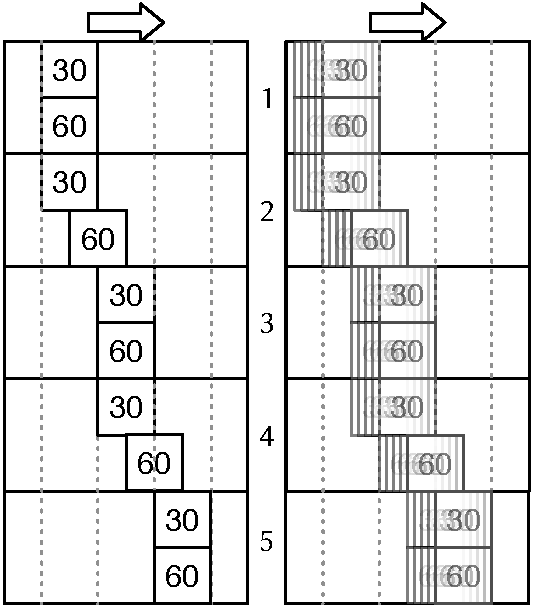
\includegraphics[width=1.0\columnwidth]{images/framerate.pdf}
% 	\caption{Effects of frame rate and motion blur on the smoothness of movement and spatial resolution. Objects move at the same speed to the right only the position os updated at different rates. A depiction of strong motion blur was added to the right-hand side.}
% \label{fig:framerate}
% \end{figure}

% The benefit of motion blur lies in its ability to conceal stutters in apparent movement due to the object and its edges being blurred, thereby reducing the positional information available on it.%, Figure~\ref{fig:framerate} illustrates this.
% Therefore, typical movie sequences usually appear to be perfectly fluid. Only for example when the camera pans at a high speed stutters in object movement or the viewport updates become apparent. Intrinsic motion blur is absent in computer generated imagery but can be artificially added to the images. While adding blur to video games can improve fluidity, it also reduces the spatial information available to the player and hampers the precision of the player's actions. Therefore it is often avoided, especially for objects in focus.

% Video games add two more factors to the frame rate consideration. The first is the issue of the monitor's refresh rate. Monitors work with a fixed, configurable image refresh rate, typically always including \SI{60}{\hertz}. If the game outputs images at an inconsistent rate or a rate lower than the monitor's refresh rate or if the framerate is not an integer multiple of the refresh rate or vice versa one of two things will happen: tearing or stuttering. % TODO: shorten and rephrase this section

% \begin{itemize}
% 	\item If the monitor fetches a frame from the graphics card's buffer while the frame is still being rendered, the result will be a mixture of the new frame in the upper half of the image and a frame which is one time interval older. This artifact is called \textbf{tearing} and should be avoided.
% 	% only the upper portion of the frame  finished, One frame split up between two refresh cycles
% 	\item Games can also be configured to postpone the rendering of a new frame until the monitor has already fetched and displayed the current frame, this is called waiting for vertical synchronization or \textbf{VSYNC}. No tearing will occur, but the \gls{IAT} of new frames might become very irregular, displaying some frames more often than others just to match the monitors refresh rate, resulting in a stuttering display. This latter stuttering effect also occurs for \SI{24}{\hertz} movies being displayed on a \SI{60}{\hertz} TV screen. Therefore most TVs additionally provide a dedicated \SI{24}{\hertz} refresh rate mode to remove the stuttering.
% \end{itemize}
